\documentclass{article}
\usepackage{graphicx} % Extended graphics inclusions
\usepackage{float}
\usepackage{url} % For \url{}
\usepackage{../config/atxy} % For front cover
\usepackage{amsfonts} % Needed for some fonts
\usepackage[usenames]{color} % Needed for colored R input/output
\usepackage{pdfcolmk} % Correct some problems with the color stack


\title{Importing sequences from ACNUC databases}

\author{Charif, D. \and Lobry, J.R.}

\usepackage{/Library/Frameworks/R.framework/Resources/share/texmf/Sweave}
\begin{document}
%
% To change the R input/output style:
%
\definecolor{Soutput}{rgb}{0,0,0.56}
\definecolor{Sinput}{rgb}{0.56,0,0}
\DefineVerbatimEnvironment{Sinput}{Verbatim}
{formatcom={\color{Sinput}},fontsize=\footnotesize, baselinestretch=0.75}
\DefineVerbatimEnvironment{Soutput}{Verbatim}
{formatcom={\color{Soutput}},fontsize=\footnotesize, baselinestretch=0.75}
%
% Rlogo
%
\newcommand{\Rlogo}{\protect
\includegraphics[height=1.8ex,keepaspectratio]{../figs/Rlogo.pdf}}
%
% Shortcut for seqinR:
%
\newcommand{\seqinr}{\texttt{seqin\bf{R}}}
\newcommand{\Seqinr}{\texttt{Seqin\bf{R}}}
\fvset{fontsize= \scriptsize}
%
% R output options and libraries to be loaded.
%
%
%  Sweave Options
%
% Put all figures in the fig folder and start the name with current file name.
% Do not produce EPS files
%


\maketitle
\tableofcontents
% BEGIN - DO NOT REMOVE THIS LINE

\section{Introduction}

As a rule of thumb, after compression one nucleotide needs one octet
of disk space storage (because you need also the annotations corresponding
to the sequences), so that most likely you won't have enough space on
your computer to work with a local copy of a complete DNA database.
The idea is to import under \Rlogo{}~only the subset of sequences you are
interested in. This is done in three steps:
\begin{enumerate}
\item Choose the bank you want to work with.
\item Select the sequences you are interested in.
\item Retrieve sequences from server into your workspace.
\end{enumerate}
We now give a full example of those three steps under the ACNUC system
\cite{GautierC1982a, GautierC1982b, acnuc1984, acnuc1985, acnuc1985b}.

\subsection{Choose a bank}

Select the database from which you want to extract sequences with the \texttt{choosebank()} function.
This function initiates a remote access to an ACNUC database. Called without arguments,
\texttt{choosebank()} returns the list of available databases:


\begin{Schunk}
\begin{Sinput}
 choosebank()
\end{Sinput}
\begin{Soutput}
 [1] "genbank"      "embl"         "emblwgs"      "swissprot"   
 [5] "ensembl"      "refseq"       "hobacnucl"    "hobacprot"   
 [9] "hovernucl"    "hoverprot"    "hogennucl"    "hogenprot"   
[13] "hogen4nucl"   "hogen4prot"   "homolensprot" "homolensnucl"
[17] "greview"      "HAMAPnucl"    "HAMAPprot"    "hoppsigen"   
[21] "nurebnucl"    "nurebprot"    "taxobacgen"  
\end{Soutput}
\end{Schunk}
 

Biological sequence databases are fast moving targets, and for publication purposes it is
recommended to specify on which release you were working on when you made the job.
To get more informations about available databases on the server, just set 
the \texttt{infobank} parameter to \texttt{TRUE}. For
instance, here is the result for the three first databases on the default server 
at the compilation time (\today) of this document:

\begin{Schunk}
\begin{Sinput}
 choosebank(infobank = TRUE)[1:3, ]
\end{Sinput}
\begin{Soutput}
     bank status
1 genbank     on
2    embl     on
3 emblwgs     on
                                                                 info
1       GenBank Rel. 162 (15 October 2007) Last Updated: Oct 30, 2007
2 EMBL Library Release 92 (September 2007) Last Updated: Oct 18, 2007
3    EMBL Whole Genome Shotgun sequences Release 92  (September 2007)
\end{Soutput}
\end{Schunk}


Note that there is a \texttt{status} column because a database could be unavailable
for a while during updates. If you try call \texttt{choosebank(bank = "bankname")} 
when the bank called \texttt{bankname} is off from server, you will get an explicit 
error message stating that this bank is temporarily unavailable, for instance:

\begin{Schunk}
\begin{Sinput}
 res <- try(choosebank("off"))
 cat(res)
\end{Sinput}
\begin{Soutput}
Error in acnucopen(bank, socket) : 
  Database with name -->off<-- is currently off for maintenance, please try again later.
\end{Soutput}
\end{Schunk}

Some special purpose databases are not listed by default. These are \textit{tagged} databases
that are only listed if you provide an explicit \texttt{tagbank} argument to the \texttt{choosebank()}
function. Of special interest for teaching purposes is the \texttt{TP} tag, an acronym for
\textit{Travaux Pratiques} which means "practicals", and corresponds to \emph{frozen}
databases so that you can set up a practical whose results are stable from year to year. Currently
available frozen databases at the default server are:

\begin{Schunk}
\begin{Sinput}
 choosebank(tagbank = "TP", infobank = TRUE)
\end{Sinput}
\begin{Soutput}
         bank status                                           info
1      emblTP     on                            frozen EMBL release
2 swissprotTP     on                       frozen SwissProt release
3 hoverprotTP     on    frozen Hovergen release - protein sequences
4 hovernuclTP     on frozen Hovergen release - nucleotide sequences
5     trypano     on                        frozen trypano database
\end{Soutput}
\end{Schunk}


Now, if you want to work with a given database, say GenBank, just call \texttt{choosebank()}
with \texttt{"genbank"} as its first argument, the result is saved in the variable
\texttt{banknameSocket} in the workspace:

\begin{Schunk}
\begin{Sinput}
 choosebank("genbank")
 str(banknameSocket)
\end{Sinput}
\begin{Soutput}
List of 9
 $ socket  :Classes 'sockconn', 'connection'  atomic [1:1] 5
  .. ..- attr(*, "conn_id")=<externalptr> 
 $ bankname: chr "genbank"
 $ banktype: chr "GENBANK"
 $ totseqs : num 82398592
 $ totspecs: num 496373
 $ totkeys : num 7273360
 $ release : chr "         GenBank Rel. 162 (15 October 2007) Last Updated: Oct 30, 2007"
 $ status  :Class 'AsIs'  chr "on"
 $ details : chr [1:4] "             ****     ACNUC Data Base Content      ****                         " "         GenBank Rel. 162 (15 October 2007) Last Updated: Oct 30, 2007" "81,770,960,650 bases; 77,863,951 sequences; 4,534,640 subseqs; 481,662 refers." "Software by M. Gouy, Lab. Biometrie et Biologie Evolutive, Universite Lyon I "
\end{Soutput}
\begin{Sinput}
 closebank()
\end{Sinput}
\end{Schunk}

The components of \texttt{banknameSocket} means that in the database
called \texttt{genbank} at the compilation time
of this document there were 
\texttt{82,398,592}
sequences from
\texttt{496,373}
species and a total of
\texttt{7,273,360}
keywords. The status of the bank was
\texttt{on}, 
and the release information was
\texttt{         GenBank Rel. 162 (15 October 2007) Last Updated: Oct 30, 2007}.
For specialized databases, some relevant informations are also given in the
\texttt{details} component, for instance:

\begin{Schunk}
\begin{Sinput}
 choosebank("taxobacgen")
 cat(banknameSocket$details, sep = "\n")
\end{Sinput}
\begin{Soutput}
               ****     ACNUC Data Base Content      ****
                 TaxoBacGen Rel. 7 (September 2005)
1,151,149,763 bases; 254,335 sequences; 847,767 subseqs; 63,879 refers.
	Data compiled from GenBank by Gregory Devulder 
        Laboratoire de Biometrie & Biologie Evolutive, Univ Lyon I
------------------------------
This database is a taxonomic genomic database. 
It results from an expertise crossing the data nomenclature database DSMZ
[http://www.dsmz.de/species/bacteria.htm Deutsche Sammlung von
Mikroorganismen und Zellkulturen GmbH, Braunschweig, Germany]
and GenBank. 
- Only contains sequences described under species present in 
Bacterial Nomenclature Up-to-date.
- Names of species and genus validly published according to the
Bacteriological Code (names with standing in nomenclature) is 
added in field "DEFINITION".
- A keyword "type strain" is added in field "FEATURES/source/strain" in
GenBank format definition to easyly identify Type Strain.
Taxobacgen is a genomic database designed for studies based on a strict
respect of up-to-date nomenclature and taxonomy.
\end{Soutput}
\begin{Sinput}
 closebank()
\end{Sinput}
\end{Schunk}

As from \seqinr~1.0-3, the result of the \texttt{choosebank()} function is automatically
stored in a global variable named \texttt{banknameSocket}, so that if no socket argument
is given to the \texttt{query()} function, the last opened database will be used by default
for your requests.
This is just a matter of convenience so that you don't have to explicitly specify the details of the
socket connection when working with the last opened database. You have, however,
full control of the process since \texttt{choosebank()} returns (invisibly) all the
required details. There is no trouble to open \emph{simultaneously} many databases.
You are just limited by the number of simultaneous connections your build of \Rlogo{}~is
allowed\footnote{
As from \Rlogo{}~2.4.0 he maximum number of open connections has been increased from
50 to 128. Note also that 
there is a very convenient function called \texttt{closeAllConnections()} in the \Rlogo{}~base package if
you want to close all open connections at once.}.

For advanced users who may wish to access to more than one database at time, a good advice
is to close them with the function \texttt{closebank()} as soon as possible so that the maximum
number of simultaneous connections is never reached. In the example below, we want to
display the number of taxa (\textit{i.e.} the number of nodes) in the species taxonomy associated
with each available database (including frozen databases). For this, we loop over available databases and 
close them as soon as the information has been retrieved.

\begin{Schunk}
\begin{Sinput}
 banks <- c(choosebank(), choosebank(tagbank = "TP"))
 nbanks <- length(banks)
 ntaxa <- numeric(nbanks)
 for (i in seq_len(nbanks)) {
     bkopenres <- try(choosebank(banks[i]))
     if (inherits(bkopenres, "try-error")) {
         ntaxa[i] <- NA
     }
     else {
         ntaxa[i] <- as.numeric(banknameSocket$totspecs)
         closebank()
     }
 }
 names(ntaxa) <- banks
\end{Sinput}
\end{Schunk}
\begin{Schunk}
\begin{Sinput}
 dotchart(log10(ntaxa[order(ntaxa)]), pch = 19, main = "Number of taxa in available databases", 
     xlab = "Log10(number of taxa)")
\end{Sinput}
\end{Schunk}
\includegraphics{../figs/getseqacnuc-plottaxaperbank}

\subsection{Make your query}

For this section, set up the default bank to GenBank, so that you don't have 
to provide the sockets details for the \texttt{query()} function:

\begin{Schunk}
\begin{Sinput}
 choosebank("genbank")
\end{Sinput}
\end{Schunk}

Then, you have to say what you want, that is to compose a query
to select the subset of sequences you are interested in. The way to do this is
documented under \texttt{?query}, we just give here a simple example. 
In the query below, we want to select all the coding sequences 
(\texttt{t=cds}) from cat (\texttt{AND sp=felis catus}) that are not 
(\texttt{AND NOT}) partial sequences (\texttt{k=partial}). 
We want the result to be stored in an object called \texttt{completeCatsCDS}.

\marginpar{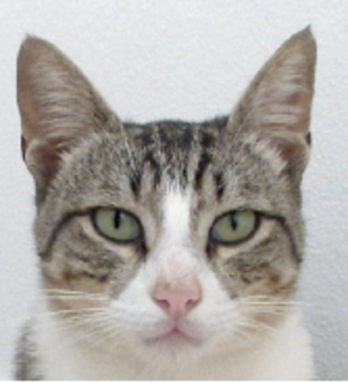
\includegraphics[width=\marginparwidth]{../figs/Feliscatus}\\
\tiny{\textit{Felis catus}. Source: wikipedia}}

\begin{Schunk}
\begin{Sinput}
 query("completeCatsCDS", "sp=felis catus AND t=cds AND NOT k=partial")
\end{Sinput}
\end{Schunk}

Now, there is in the workspace an object called \texttt{completeCatsCDS}, which
does not contain the sequences themselves but the \emph{sequence names} (and various relevant informations
such as the genetic code and the frame) that fit 
the query. They are stored in the \texttt{req} component of the object,
let's see the name of the first ten of them:

\begin{Schunk}
\begin{Sinput}
 sapply(completeCatsCDS$req[1:10], getName)
\end{Sinput}
\begin{Soutput}
 [1] "AB000483.PE1"    "AB000484.PE1"    "AB000485.PE1"    "AB004237"       
 [5] "AB004238"        "AB009279.PE1"    "AB009280.PE1"    "AB010872.UGT1A1"
 [9] "AB011965.SDF-1A" "AB011966.SDF-1B"
\end{Soutput}
\end{Schunk}

The first sequence that fit our request is \texttt{AB000483.PE1},
the second one is \texttt{AB000484.PE1}, and so on. Note that
the sequence name may have an extension, this corresponds to \emph{subsequences},
a specificity of the ACNUC system that allows to handle easily a
subsequence with a biological meaning, typically a gene. The list of available subsequences
in a given database is given by the function \texttt{getType()}, for example the list
of available subsequences in GenBank is given in table \ref{genbank}.

%
% Besoin d'edition manuelle du fichier genbank.tex pour virer les caracteres sp�ciaux Latex, ici "_"
%
% latex table generated in R 2.1.0 by xtable 1.2-5 package
% Wed Jul 20 12:00:16 2005
\begin{table}[ht]
\begin{center}
\begin{tabular}{rll}
\hline
 & Type & Description \\
\hline
1 &      CDS &              .PE protein coding region \\
2 &    LOCUS &                 sequenced DNA fragment \\
3 & MISC\_RNA & .RN other structural RNA coding region \\
4 &     RRNA &               .RR mature ribosomal RNA \\
5 &    SCRNA &              .SC small cytoplasmic RNA \\
6 &    SNRNA &                  .SN small nuclear RNA \\
7 &     TRNA &                .TR mature transfer RNA \\
\hline
\end{tabular}
\caption{Available subsequences in genbank}
\label{genbank}
\end{center}
\end{table}



The component \texttt{call} of \texttt{completeCatsCDS} keeps automatically a 
trace of the way you have selected the sequences: 

\begin{Schunk}
\begin{Sinput}
 completeCatsCDS$call
\end{Sinput}
\begin{Soutput}
query(listname = "completeCatsCDS", query = "sp=felis catus AND t=cds AND NOT k=partial")
\end{Soutput}
\end{Schunk}

At this stage you can quit your \Rlogo{} 
session saving the workspace image. The next time an \Rlogo{}~session is opened with the 
workspace image restored, there will be an object called \texttt{completeCatsCDS}, and 
looking into its \texttt{call} component will tell you that it contains the names 
of complete coding sequences from \textit{Felis catus}.

In practice, queries for sequences are rarely done in one step and are more likely
to be the result of an iterative, progressively refining, process. An important point
is that a list of sequences can be re-used. For instance, we can re-use \texttt{completeCatsCDS}
to get only the list of sequences that were published in 2004:

\begin{Schunk}
\begin{Sinput}
 query("ccc2004", "completeCatsCDS AND y=2004")
 length(ccc2004$req)
\end{Sinput}
\begin{Soutput}
[1] 58
\end{Soutput}
\end{Schunk}

Hence, there were 58 complete coding sequences published in 2004 for
\textit{Felis catus} in GenBank.

As from release 1.0-3 of the \seqinr{} package, there is new parameter \texttt{virtual}
which allows to disable the automatic retrieval of information for all list elements. This is interesting for list
with many elements, for instance :

\begin{Schunk}
\begin{Sinput}
 query("allcds", "t=cds", virtual = TRUE)
 allcds$nelem
\end{Sinput}
\begin{Soutput}
[1] 4857947
\end{Soutput}
\end{Schunk}

There are therefore \texttt{4,857,947} coding
sequences in this version of GenBank\footnote{
which is stored in the \texttt{release} component of the object \texttt{banknameSocket}
and current value is today (\today): \texttt{banknameSocket\$release = 
         GenBank Rel. 162 (15 October 2007) Last Updated: Oct 30, 2007}.
}. 
It would be long to get all the informations for the elements
of this list, so we have set the parameter \texttt{virtual} to \texttt{TRUE} and the \texttt{req}
component of the list has not been documented:

\begin{Schunk}
\begin{Sinput}
 allcds$req
\end{Sinput}
\begin{Soutput}
[1] NA
\end{Soutput}
\end{Schunk}

However, the list can still be re-used\footnote{
of course, as long as the socket connection with the server has not been lost: virtual lists details are only
known by the server.}, 
for instance we may extract from this list all the sequences
from, say, \textit{Mycoplasma genitalium}:

\begin{Schunk}
\begin{Sinput}
 query("small", "allcds AND sp=mycoplasma genitalium", virtual = TRUE)
 small$nelem
\end{Sinput}
\begin{Soutput}
[1] 931
\end{Soutput}
\end{Schunk}

There are then \texttt{931} elements in
the list \texttt{small}, so that we can safely repeat the previous query without asking for a
virtual list:

\begin{Schunk}
\begin{Sinput}
 query("small", "allcds et sp=mycoplasma genitalium")
 sapply(small$req, getName)[1:10]
\end{Sinput}
\begin{Soutput}
 [1] "AY191424" "AY386807" "AY386808" "AY386809" "AY386810" "AY386811"
 [7] "AY386812" "AY386813" "AY386814" "AY386815"
\end{Soutput}
\end{Schunk}

Here are some illustrations of using virtual list to answer simple questions about the
current GenBank release.

\begin{description}
\item[\textbf{Man.}] How many sequences are available for our species?
\begin{Schunk}
\begin{Sinput}
 query("man", "sp=homo sapiens", virtual = T)
 man$nelem
\end{Sinput}
\begin{Soutput}
[1] 11260600
\end{Soutput}
\end{Schunk}
There are \texttt{11,260,600} sequences from \textit{Homo sapiens}.

\item[\textbf{Sex.}] How many sequences are annotated with a keyword starting by sex?
\begin{Schunk}
\begin{Sinput}
 query("sex", "k=sex@", virtual = T)
 sex$nelem
\end{Sinput}
\begin{Soutput}
[1] 1196
\end{Soutput}
\end{Schunk}
There are \texttt{1,196} such sequences.

\item[\textbf{tRNA.}] How many complete tRNA sequences are available?
\begin{Schunk}
\begin{Sinput}
 query("trna", "t=trna AND NOT k=partial", virtual = T)
 trna$nelem
\end{Sinput}
\begin{Soutput}
[1] 254050
\end{Soutput}
\end{Schunk}
There are \texttt{254,050} complete tRNA sequences.

\item[\textbf{Nature vs. Science.}] In which journal were the more sequences published?
\begin{Schunk}
\begin{Sinput}
 query("nature", "j=nature", virtual = T)
 nature$nelem
\end{Sinput}
\begin{Soutput}
[1] 1533556
\end{Soutput}
\begin{Sinput}
 query("science", "j=science", virtual = T)
 science$nelem
\end{Sinput}
\begin{Soutput}
[1] 1284219
\end{Soutput}
\end{Schunk}
There are \texttt{1,533,556} sequences published
in \textit{Nature} and
\texttt{1,284,219} sequences published in
\textit{Science}, so that the winner is 
\textit{Nature}.

%
% \item[TriTryp] quand la ref de Science/309/404 sera dans genbank
%

\item[\textbf{Smith.}] How many sequences have Smith (last name) as author?
\begin{Schunk}
\begin{Sinput}
 query("smith", "au=smith", virtual = T)
 smith$nelem
\end{Sinput}
\begin{Soutput}
[1] 4107145
\end{Soutput}
\end{Schunk}
There are \texttt{4,107,145} such sequences.

\item[\textbf{YK2.}] How many sequences were published after year 2000 (included)?
\begin{Schunk}
\begin{Sinput}
 query("yk2", "y>2000", virtual = T)
 yk2$nelem
\end{Sinput}
\begin{Soutput}
[1] 66366478
\end{Soutput}
\end{Schunk}
There are \texttt{66,366,478} sequences published after year 2000.

\item[\textbf{Organelle contest.}] Do we have more sequences from chloroplast genomes or from mitochondion genomes?
\begin{Schunk}
\begin{Sinput}
 query("chloro", "o=chloroplast", virtual = T)
 chloro$nelem
\end{Sinput}
\begin{Soutput}
[1] 151023
\end{Soutput}
\begin{Sinput}
 query("mito", "o=mitochondrion", virtual = T)
 mito$nelem
\end{Sinput}
\begin{Soutput}
[1] 516327
\end{Soutput}
\end{Schunk}
There are \texttt{151,023} sequences from
chloroplast genomes and
\texttt{516,327} sequences from mitochondrion
genomes, so that the winner is 
mitochondrion.


\end{description}

\begin{Schunk}
\begin{Sinput}
 closebank()
\end{Sinput}
\end{Schunk}


\subsection{Extract sequences of interest}

\subsubsection{Introduction}

There are two functions to get the sequences. The first one, 
\texttt{getSequence()}, uses regular socket connections, the
second one, \texttt{extractseq()}, uses zlib compressed sockets,
which is faster but the function is experimental and has not
been extensively tested.

\subsubsection{Extacting sequences with \texttt{getSequence()}}


For this section we set up the bank to \texttt{emblTP} which is a frozen
subset of EMBL database to allow for the reproducibility of results.

\begin{Schunk}
\begin{Sinput}
 choosebank("emblTP")
\end{Sinput}
\end{Schunk}

We suppose that the sequences we are interested in are all the complete
coding sequences from \textit{Felis catus} :

\begin{Schunk}
\begin{Sinput}
 query("completeCatsCDS", "sp=felis catus AND t=cds AND NOT k=partial")
 (nseq <- completeCatsCDS$nelem)
\end{Sinput}
\begin{Soutput}
[1] 257
\end{Soutput}
\end{Schunk}

Thus, there were 257 complete
CDS from \textit{Felis catus} in this release of EMBL.


The sequences are obtained with the function \texttt{getSequence()}.
For example, the first 50 nucleotides of the first sequence of our request are:

\begin{Schunk}
\begin{Sinput}
 myseq <- getSequence(completeCatsCDS$req[[1]])
 myseq[1:50]
\end{Sinput}
\begin{Soutput}
 [1] "a" "t" "g" "a" "c" "c" "a" "a" "c" "a" "t" "t" "c" "g" "a" "a" "a" "a"
[19] "t" "c" "a" "c" "a" "c" "c" "c" "c" "c" "t" "t" "a" "c" "c" "a" "a" "a"
[37] "a" "t" "t" "a" "t" "t" "a" "a" "t" "c" "a" "c" "t" "c"
\end{Soutput}
\end{Schunk}
They can also be coerced as string of character with the function \texttt{c2s()}:
\begin{Schunk}
\begin{Sinput}
 c2s(myseq[1:50])
\end{Sinput}
\begin{Soutput}
[1] "atgaccaacattcgaaaatcacacccccttaccaaaattattaatcactc"
\end{Soutput}
\end{Schunk}

Note that what is done by \texttt{getSequence()} is much more complex
than a substring extraction because subsequences of biological interest are
not necessarily contiguous or even on the same DNA strand. Consider for
instance the following coding sequence from sequence \texttt{AE003734}:

\begin{Schunk}
\begin{Sinput}
 query("trs", "N=AE003734.PE35")
 annots <- getAnnot(trs$req[[1]])
 cat(annots, sep = "\n")
\end{Sinput}
\begin{Soutput}
FT   CDS             join(complement(153944..154157),complement(153727..153866),
FT                   complement(152185..153037),138523..138735,138795..138955)
FT                   /codon_start=1
FT                   /db_xref="FLYBASE:FBgn0002781"
FT                   /db_xref="GOA:Q86B86"
FT                   /db_xref="TrEMBL:Q86B86"
FT                   /note="mod(mdg4) gene product from transcript CG32491-RZ;
FT                   trans splicing"
FT                   /gene="mod(mdg4)"
FT                   /product="CG32491-PZ"
FT                   /locus_tag="CG32491"
FT                   /protein_id="AAO41581.1"
FT                   /translation="MADDEQFSLCWNNFNTNLSAGFHESLCRGDLVDVSLAAEGQIVKA
FT                   HRLVLSVCSPFFRKMFTQMPSNTHAIVFLNNVSHSALKDLIQFMYCGEVNVKQDALPAF
FT                   ISTAESLQIKGLTDNDPAPQPPQESSPPPAAPHVQQQQIPAQRVQRQQPRASARYKIET
FT                   VDDGLGDEKQSTTQIVIQTTAAPQATIVQQQQPQQAAQQIQSQQLQTGTTTTATLVSTN
FT                   KRSAQRSSLTPASSSAGVKRSKTSTSANVMDPLDSTTETGATTTAQLVPQQITVQTSVV
FT                   SAAEAKLHQQSPQQVRQEEAEYIDLPMELPTKSEPDYSEDHGDAAGDAEGTYVEDDTYG
FT                   DMRYDDSYFTENEDAGNQTAANTSGGGVTATTSKAVVKQQSQNYSESSFVDTSGDQGNT
FT                   EAQVTQHVRNCGPQMFLISRKGGTLLTINNFVYRSNLKFFGKSNNILYWECVQNRSVKC
FT                   RSRLKTIGDDLYVTNDVHNHMGDNKRIEAAKAAGMLIHKKLSSLTAADKIQGSWKMDTE
FT                   GNPDHLPKM"
\end{Soutput}
\end{Schunk}


To get the coding sequence manually you would have join 5 different pieces 
from \texttt{AE003734} and some of them are in the complementary strand. 
With \texttt{getSequence()} you don't have to think about this. Just make a
query with the sequence name:

\begin{Schunk}
\begin{Sinput}
 query("transspliced", "N=AE003734.PE35")
 length(transspliced$req)
\end{Sinput}
\begin{Soutput}
[1] 1
\end{Soutput}
\begin{Sinput}
 getName(transspliced$req[[1]])
\end{Sinput}
\begin{Soutput}
[1] "AE003734.PE35"
\end{Soutput}
\end{Schunk}

Ok, now there is in your workspace an object called \texttt{transspliced} which \texttt{req}
component is of length one (because you have asked for just one sequence) and the name of the
single element of the req component is AE003734.PE35 (because this
is the name of the sequence you wanted). Let see the first 50 base of this sequence:

\begin{Schunk}
\begin{Sinput}
 getSequence(transspliced$req[[1]])[1:50]
\end{Sinput}
\begin{Soutput}
 [1] "a" "t" "g" "g" "c" "g" "g" "a" "c" "g" "a" "c" "g" "a" "g" "c" "a" "a"
[19] "t" "t" "c" "a" "g" "c" "t" "t" "g" "t" "g" "c" "t" "g" "g" "a" "a" "c"
[37] "a" "a" "c" "t" "t" "c" "a" "a" "c" "a" "c" "g" "a" "a"
\end{Soutput}
\end{Schunk}

All the complex transsplicing operations have been done here. You can check that there is no
in-frame stop codons\footnote{
Stop codons are represented by the character \texttt{*} when translated into protein.} 
with the \texttt{getTrans()} function to translate this coding sequence into protein:

\begin{Schunk}
\begin{Sinput}
 getTrans(transspliced$req[[1]])[1:50]
\end{Sinput}
\begin{Soutput}
 [1] "M" "A" "D" "D" "E" "Q" "F" "S" "L" "C" "W" "N" "N" "F" "N" "T" "N" "L"
[19] "S" "A" "G" "F" "H" "E" "S" "L" "C" "R" "G" "D" "L" "V" "D" "V" "S" "L"
[37] "A" "A" "E" "G" "Q" "I" "V" "K" "A" "H" "R" "L" "V" "L"
\end{Soutput}
\begin{Sinput}
 table(getTrans(transspliced$req[[1]]))
\end{Sinput}
\begin{Soutput}
 *  A  C  D  E  F  G  H  I  K  L  M  N  P  Q  R  S  T  V  W  Y 
 1 47  7 33 25 15 29 12 20 26 33 12 27 25 52 19 48 47 34  3 12 
\end{Soutput}
\end{Schunk}

In a more graphical way:

\begin{Schunk}
\begin{Sinput}
 aacount <- table(getTrans(transspliced$req[[1]]))
 aacount <- aacount[order(aacount)]
 names(aacount) <- aaa(names(aacount))
 dotchart(aacount, pch = 19, xlab = "Stop and amino-acid counts", 
     main = "There is only one stop codon in AE003734.PE35")
 abline(v = 1, lty = 2)
\end{Sinput}
\end{Schunk}
\includegraphics{../figs/getseqacnuc-transp4}

Note that the relevant variant of the genetic code was automatically set up during the translation
of the sequence into protein. This is because the \texttt{transspliced\$req[[1]]} object belongs to the 
\texttt{SeqAcnucWeb} class:

\begin{Schunk}
\begin{Sinput}
 class(transspliced$req[[1]])
\end{Sinput}
\begin{Soutput}
[1] "SeqAcnucWeb"
\end{Soutput}
\end{Schunk}

Therefore, when you are using the \texttt{getTrans()} function, you are automatically redirected
to the \texttt{getTrans.SeqAcnucWeb()} function which knows how to take into account the relevant frame
and genetic code for your coding sequence.

\begin{Schunk}
\begin{Sinput}
 closebank()
\end{Sinput}
\end{Schunk}

\subsubsection{Extacting sequences with \texttt{extractseqs()} (experimental)}

The timings here were from an home-ADSL connection, and are only indicative.
For this section we set up the bank to \texttt{emblTP} which is a frozen
subset of EMBL database to allow for the reproducibility of results.

%
% For some reason I don't understand all these should be in the same code chunk:
%
\begin{Schunk}
\begin{Sinput}
 rm(list = ls(all = TRUE))
 gc()
\end{Sinput}
\begin{Soutput}
         used (Mb) gc trigger  (Mb) max used  (Mb)
Ncells 244254  6.6    4195948 112.1  5860551 156.5
Vcells 570263  4.4   29477531 224.9 37726935 287.9
\end{Soutput}
\begin{Sinput}
 (tcb <- system.time(choosebank("emblTP")))
\end{Sinput}
\begin{Soutput}
utilisateur    syst`eme    'ecoul'e 
      0.059       0.001       5.392 
\end{Soutput}
\begin{Sinput}
 (tqu <- system.time(query("hsCDS", "sp=Homo sapiens AND t=cds AND o=nuclear AND NOT k=partial", 
     virtual = TRUE)))
\end{Sinput}
\begin{Soutput}
utilisateur    syst`eme    'ecoul'e 
      0.001       0.000      11.256 
\end{Soutput}
\begin{Sinput}
 (nseq <- hsCDS$nelem)
\end{Sinput}
\begin{Soutput}
[1] 78573
\end{Soutput}
\begin{Sinput}
 showConnections()
\end{Sinput}
\begin{Soutput}
  description                 class    mode text   isopen   can read
3 "getseqacnuc.tex"           "file"   "w+" "text" "opened" "yes"   
4 ""                          "file"   "w+" "text" "opened" "yes"   
5 "->pbil.univ-lyon1.fr:5558" "socket" "a+" "text" "opened" "yes"   
  can write
3 "yes"    
4 "yes"    
5 "yes"    
\end{Soutput}
\begin{Sinput}
 Sys.sleep(1)
 (tex <- system.time(mycds <- extractseqs("hsCDS", verbose = TRUE)))
\end{Sinput}
\begin{Soutput}
I'm checking the arguments...
... and everything is OK up to now.
Format is  fasta 
Operation is  simple 
The rank of the list  hsCDS is  2 .
request :  extractseqs&lrank=2&format=fasta&operation=simple&zlib=T 
Running getzlibsock... 
'con' is a connection...
Socket number is 5....
Trying to get answer from socket...

-->[code=0]
Socket answer is ok code=0(6)
n=1000, nn=1000,nnn=1000
Increasing memory...
Increasing memory...
Increasing memory...
Increasing memory...
Increasing memory...
Increasing memory...
Increasing memory...
Increasing memory...
Increasing memory...
Increasing memory...
Increasing memory...
extractseqs successfully ended ...
Number of lines     : 1799153
Number of sequences : 78573
extractseqs OK, program carry on...
Ok, everything is fine!
Closing socket close_sock_gz_r  status = 0
utilisateur    syst`eme    'ecoul'e 
      9.024       1.121      60.955 
\end{Soutput}
\end{Schunk}

It was then about 5 
seconds to select
the relevant database. We suppose that the sequences we are interested in 
are all the complete coding sequences from \textit{Homo sapiens} that
are encoded in the nucleus (we don't want sequences from human mitochondrion). 
We have used a virtual query to speed up things:
it was about 11 seconds 
to create on the server a list of 78573
sequences. We have downloaded the sequences in zlib compressed mode:
it was about 61 seconds
to dowload the sequences in the object \texttt{mycds}, which looks like :

\begin{Schunk}
\begin{Sinput}
 cat(head(mycds), sep = "\n")
\end{Sinput}
\begin{Soutput}
>A00127.PE1             2217 residues
ATGCGGGGTCCGAGCGGGGCTCTGTGGCTGCTCCTGGCTCTGCGCACCGTGCTCGGAGGC
ATGGAGGTGCGGTGGTGCGCCACCTCGGACCCAGAGCAGCACAAGTGCGGCAACATGAGC
GAGGCCTTCCGGGAAGCGGGCATCCAGCCCTCCCTCCTCTGCGTCCGGGGCACCTCCGCC
GACCACTGCGTCCAGCTCATCGCGGCCCAGGAGGCTGACGCCATCACTCTGGATGGAGGA
GCCATCTATGAGGCGGGAAAGGAGCACGGCCTGAAGCCGGTGGTGGGCGAAGTGTACGAT
\end{Soutput}
\begin{Sinput}
 cat(tail(mycds), sep = "\n")
\end{Sinput}
\begin{Soutput}
ATCACTGCGGCCCCAGAGAGAGAGGGCATAGGCCACGGCGGCCCCAAGCTATGCTGCACA
CTGAGCTCCCTCAGCTCCGCTGCTGAGACTGGCCGGGACCCGCTGGACAGCGAGGAGGAG
GCAACCAGCGGCGCCCAGGATGAACGTGGCCTGAAGCCGCCTTCCCGGGGCCAGTTTCCT
TCCCTCTCAGCCAGGGATGCCTCGAGCAGCCACAGGGGCAGGAACGTCCTGACTGCCATC
CTGCTGCTGCTGCGGGAGCTGGATGCAGAGGGGCTGGAGGCCGTGCAGCAGACTGTGGGC
AGCCGGCTGCAGGCCCTGCGTGGGGAAGAGGTGCAGGAGCACGCCGAGTGA
\end{Soutput}
\end{Schunk}

We save now the sequences in a local FASTA file for future use:

\begin{Schunk}
\begin{Sinput}
 (twl <- system.time(writeLines(mycds, "mycds.fasta")))
\end{Sinput}
\begin{Soutput}
utilisateur    syst`eme    'ecoul'e 
      0.875       0.791       2.764 
\end{Soutput}
\end{Schunk}

It was then about 3 seconds
to dump the sequences on a local file. We read the sequences as strings
without setting attributes to save time:

\begin{Schunk}
\begin{Sinput}
 (trf <- system.time(mycdss <- read.fasta("mycds.fasta", as.string = TRUE, 
     set.attributes = FALSE)))
\end{Sinput}
\begin{Soutput}
utilisateur    syst`eme    'ecoul'e 
     34.280       0.308      34.792 
\end{Soutput}
\end{Schunk}

It was then about 35 seconds
to read the sequences as strings. We save them in XDR format:

\begin{Schunk}
\begin{Sinput}
 (tsrd <- system.time(save(mycdss, file = "mycdss.RData")))
\end{Sinput}
\begin{Soutput}
utilisateur    syst`eme    'ecoul'e 
     38.849       0.338      39.813 
\end{Soutput}
\end{Schunk}

It was then about 40 seconds
to save the sequences in XDR format. How long is it to load the sequences
from XDR format?

\begin{Schunk}
\begin{Sinput}
 (tlrd <- system.time(load("mycdss.RData")))
\end{Sinput}
\begin{Soutput}
utilisateur    syst`eme    'ecoul'e 
      1.764       0.041       1.813 
\end{Soutput}
\end{Schunk}

It was then about 2 seconds
to load the sequences from an XDR formated file. Now, we also want the
corresponding proteins. We download the translated CDS from the server:

\begin{Schunk}
\begin{Sinput}
 (texp <- system.time(myprot <- extractseqs("hsCDS", operation = "translate")))
\end{Sinput}
\begin{Soutput}
utilisateur    syst`eme    'ecoul'e 
      3.680       0.647      60.748 
\end{Soutput}
\end{Schunk}

It was then about 61 seconds
to get the protein sequences from the server. The object \texttt{myprot} looks
like:

\begin{Schunk}
\begin{Sinput}
 cat(head(myprot), sep = "\n")
\end{Sinput}
\begin{Soutput}
>A00127.PE1              739 residues
MRGPSGALWLLLALRTVLGGMEVRWCATSDPEQHKCGNMSEAFREAGIQPSLLCVRGTSA
DHCVQLIAAQEADAITLDGGAIYEAGKEHGLKPVVGEVYDQEVGTSYYAVAVVRRSSHVT
IDTLKGVKSCHTGINRTVGWNVPVGYLVESGRLSVMGCDVLKAVSDYFGGSCVPGAGETS
YSESLCRLCRGDSSGEGVCDKSPLERYYDYSGAFRCLAEGAGDVAFVKHSTVLENTDGKT
LPSWGQALLSQDFELLCRDGSRADVTEWRQCHLARVPAHAVVVRADTDGGLIFRLLNEGQ
\end{Soutput}
\begin{Sinput}
 cat(tail(myprot), sep = "\n")
\end{Sinput}
\begin{Soutput}
>Z93322.PE1              257 residues
MKLTRKMVLTRAKASELHSVRKLNCWGSRLTDISICQEMPSLEVITLSVNSISTLEPVSR
CQRLSELYLRRNRIPSLAELFYLKGLPRLRVLWLAENPCCGTSPHRYRMTVLRTLPRLQK
LDNQAVTEEELSRALSEGEEITAAPEREGIGHGGPKLCCTLSSLSSAAETGRDPLDSEEE
ATSGAQDERGLKPPSRGQFPSLSARDASSSHRGRNVLTAILLLLRELDAEGLEAVQQTVG
SRLQALRGEEVQEHAE*
\end{Soutput}
\end{Schunk}

We save the protein sequences in a local FASTA file for future use:

\begin{Schunk}
\begin{Sinput}
 (twl2 <- system.time(writeLines(myprot, "myprot.fasta")))
\end{Sinput}
\begin{Soutput}
utilisateur    syst`eme    'ecoul'e 
      0.330       0.274       0.605 
\end{Soutput}
\end{Schunk}

It was then about 1 seconds
to dump the protein sequences on a local file. We read the sequences as strings
without setting attributes to save time:

\begin{Schunk}
\begin{Sinput}
 (trf2 <- system.time(myprots <- read.fasta("myprot.fasta", 
     as.string = TRUE, set.attributes = FALSE)))
\end{Sinput}
\begin{Soutput}
utilisateur    syst`eme    'ecoul'e 
     22.588       0.148      22.859 
\end{Soutput}
\end{Schunk}

It was then about 23 seconds
to read the protein sequences as strings. We save them in XDR format:

\begin{Schunk}
\begin{Sinput}
 (tsrd2 <- system.time(save(myprots, file = "myprots.RData")))
\end{Sinput}
\begin{Soutput}
utilisateur    syst`eme    'ecoul'e 
      3.766       0.154       4.282 
\end{Soutput}
\end{Schunk}

It was then about 4 seconds
to save the protein sequences in XDR format. How long is it to load the 
protein sequences from XDR format?

\begin{Schunk}
\begin{Sinput}
 (tlrd2 <- system.time(load("myprots.RData")))
\end{Sinput}
\begin{Soutput}
utilisateur    syst`eme    'ecoul'e 
      1.092       0.027       1.121 
\end{Soutput}
\end{Schunk}

It was then about 1 seconds
to load the protein sequences from an XDR formated file.

%Summary in a table -- bof bof

As a quick sanity check, we plot the distribution of protein size:

\setkeys{Gin}{width=\textwidth}

\begin{Schunk}
\begin{Sinput}
 x <- log10(nchar(myprots) - 1)
 dstx <- density(x)
 plot(dstx, main = paste("Protein size distribution in the human genome\nn = ", 
     length(myprots), "proteins"), xlab = "Number of amino-acids in log 10 scale", 
     las = 1)
 rug(x, col = "blue")
 polycurve <- function(x, y, base.y = min(y), ...) polygon(x = c(min(x), 
     x, max(x)), y = c(base.y, y, base.y), ...)
 polycurve(dstx$x, dstx$y, col = "yellow")
\end{Sinput}
\end{Schunk}
\includegraphics{../figs/getseqacnuc-protsizeinhuman}

\begin{Schunk}
\begin{Sinput}
 closebank()
\end{Sinput}
\end{Schunk}

\section{The query language}


\subsection{Where to find information}

The last version of the documentation for the query language is available online
at \url{http://pbil.univ-lyon1.fr/databases/acnuc/cfonctions.html#QUERYLANGUAGE}.
This documentation has been imported within the documentation of the
\texttt{query()} function, but the last available update is the online version.

\subsection{Case sensitivity and ambiguities resolution}

The query language is case insensitive, for instance:

\begin{Schunk}
\begin{Sinput}
 choosebank("emblTP")
 query("lowercase", "sp=escherichia coli", virtual = TRUE)
 query("uppercase", "SP=Escherichia coli", virtual = TRUE)
 lowercase$nelem == uppercase$nelem
\end{Sinput}
\begin{Soutput}
[1] TRUE
\end{Soutput}
\begin{Sinput}
 closebank()
\end{Sinput}
\end{Schunk}

Three operators (AND, OR, NOT) 
can be ambiguous because they can also occur within valid criterion values. 
Such ambiguities can be solved by encapsulating elementary selection 
criteria between escaped double quotes. For example:

\begin{Schunk}
\begin{Sinput}
 choosebank("emblTP")
 query("ambig", "\"sp=Beak and feather disease virus\" AND \"au=ritchie\"", 
     virtual = T)
 ambig$nelem
\end{Sinput}
\begin{Soutput}
[1] 18
\end{Soutput}
\begin{Sinput}
 closebank()
\end{Sinput}
\end{Schunk}

\subsection{Selection criteria}

\subsubsection{Introduction}

Selection criteria are in the form \texttt{c=something} (without space
before the = sign) or \texttt{list\_name} where \texttt{list\_name} is a
previously constructed list.

\subsubsection{\texttt{SP=taxon}}

This is used to select sequences attached to a given taxon or any other below in
the tree. The at sign @ substitutes as a wildcard character for any zero or more 
characters. Here are some examples:

\begin{Schunk}
\begin{Sinput}
 choosebank("emblTP")
 query("bb", "sp=Borrelia burgdorferi", virtual = T)
 bb$nelem
\end{Sinput}
\begin{Soutput}
[1] 1682
\end{Soutput}
\begin{Sinput}
 query("borrelia", "sp=Borrelia", virtual = T)
 borrelia$nelem
\end{Sinput}
\begin{Soutput}
[1] 3173
\end{Soutput}
\begin{Sinput}
 closebank()
\end{Sinput}
\end{Schunk}

Here is an example of use of the wildcard @ to look for sapiens species:

\begin{Schunk}
\begin{Sinput}
 choosebank("emblTP")
 query("sapiens", "sp=@sapiens@", virtual = T)
 sapiens$nelem
\end{Sinput}
\begin{Soutput}
[1] 2216556
\end{Soutput}
\begin{Sinput}
 query("sapienspecies", "PS sapiens")
 sapply(sapienspecies$req, getName)
\end{Sinput}
\begin{Soutput}
 [1] "HOMO SAPIENS"                            
 [2] "HOMO SAPIENS NEANDERTHALENSIS"           
 [3] "HOMO SAPIENS X HUMAN PAPILLOMAVIRUS TYPE"
 [4] "HOMO SAPIENS X SIMIAN VIRUS 40"          
 [5] "HOMO SAPIENS X HUMAN ENDOGENOUS RETROVIR"
 [6] "HOMO SAPIENS X HUMAN T-CELL LYMPHOTROPIC"
 [7] "HEPATITIS B VIRUS X HOMO SAPIENS"        
 [8] "HOMO SAPIENS X HEPATITIS B VIRUS"        
 [9] "HOMO SAPIENS X HUMAN IMMUNODEFICIENCY VI"
[10] "SYNTHETIC CONSTRUCT X HOMO SAPIENS"      
[11] "HUMAN PAPILLOMAVIRUS X HOMO SAPIENS"     
[12] "MUS SP. X HOMO SAPIENS"                  
[13] "HOMO SAPIENS X HUMAN PAPILLOMAVIRUS"     
[14] "HOMO SAPIENS X HUMAN ADENOVIRUS TYPE 5"  
[15] "HOMO SAPIENS X HERV-H/ENV62"             
[16] "HOMO SAPIENS X HERV-H/ENV60"             
[17] "HOMO SAPIENS X HERV-H/ENV59"             
[18] "EXPRESSION VECTOR PTH-HIN X HOMO SAPIENS"
[19] "ADENO-ASSOCIATED VIRUS 2 X HOMO SAPIENS" 
[20] "SIMIAN VIRUS 40 X HOMO SAPIENS"          
[21] "HOMO SAPIENS X MUS MUSCULUS"             
[22] "HOMO SAPIENS X INFLUENZA B VIRUS (B/LEE/"
[23] "MUS MUSCULUS X HOMO SAPIENS"             
[24] "CRICETULUS GRISEUS X HOMO SAPIENS"       
[25] "TRYPANOSOMA CRUZI X HOMO SAPIENS"        
[26] "HOMO SAPIENS X TRYPANOSOMA CRUZI"        
\end{Soutput}
\begin{Sinput}
 closebank()
\end{Sinput}
\end{Schunk}

\subsubsection{\texttt{TID=id}}

This is used to select sequences attached attached to a given numerical 
NCBI's taxonomy ID. For instance, the taxonomy ID for 
\textit{Homo sapiens neanderthalensis} is 63221:

\marginpar{
\includegraphics[width=\marginparwidth]{../figs/hsn}\\
\tiny{\textit{Homo neanderthalensis}. Source: wikipedia}}

\begin{Schunk}
\begin{Sinput}
 choosebank("genbank")
 query("hsn", "TID=63221", virtual = T)
 hsn$nelem
\end{Sinput}
\begin{Soutput}
[1] 1337
\end{Soutput}
\begin{Sinput}
 query("hsnsp", "PS hsn")
 sapply(hsnsp$req, getName)
\end{Sinput}
\begin{Soutput}
[1] "HOMO SAPIENS NEANDERTHALENSIS"
\end{Soutput}
\begin{Sinput}
 closebank()
\end{Sinput}
\end{Schunk}

\subsubsection{\texttt{K=keyword}}

This is used to select sequences attached to a given keyword or any other below in
the tree. The at sign @ substitutes as a wildcard character for any zero or more 
characters. Example:

\begin{Schunk}
\begin{Sinput}
 choosebank("emblTP")
 query("ecoliribprot", "sp=escherichia coli AND k=rib@ prot@", 
     virtual = T)
 ecoliribprot$nelem
\end{Sinput}
\begin{Soutput}
[1] 105
\end{Soutput}
\begin{Sinput}
 closebank()
\end{Sinput}
\end{Schunk}

\subsubsection{\texttt{T=type}}

This is used to select sequences of specified type. The list of available
type for the currently opened database is given by function \texttt{getType()}:

\begin{Schunk}
\begin{Sinput}
 choosebank("emblTP")
 getType()
\end{Sinput}
\begin{Soutput}
        sname                                  libel
2661      CDS              .PE protein coding region
2662       ID                            Locus entry
2663 MISC_RNA .RN other structural RNA coding region
2664     RRNA          .RR Ribosomal RNA coding gene
2665    SCRNA              .SC small cytoplasmic RNA
2666    SNRNA                  .SN small nuclear RNA
2667     TRNA           .TR Transfer RNA coding gene
\end{Soutput}
\begin{Sinput}
 closebank()
\end{Sinput}
\end{Schunk}

For instance, to select all coding sequences from \textit{Homo sapiens} we can use:

\begin{Schunk}
\begin{Sinput}
 choosebank("emblTP")
 query("hscds", "sp=Homo sapiens AND t=cds", virtual = T)
 hscds$nelem
\end{Sinput}
\begin{Soutput}
[1] 150513
\end{Soutput}
\begin{Sinput}
 closebank()
\end{Sinput}
\end{Schunk}

\subsubsection{\texttt{J=journal\_name}}

This is used to select sequences published in journal specified using defined journal code.
For instance to select all sequences published in \textit{Science}:

\begin{Schunk}
\begin{Sinput}
 choosebank("emblTP")
 query("allseqsfromscience", "J=Science", virtual = TRUE)
 allseqsfromscience$nelem
\end{Sinput}
\begin{Soutput}
[1] 930397
\end{Soutput}
\begin{Sinput}
 closebank()
\end{Sinput}
\end{Schunk}

The list of available journal code can be obtained from the \texttt{readsmj()} function
this way:

\begin{Schunk}
\begin{Sinput}
 choosebank("emblTP")
 nl <- readfirstrec(type = "SMJ")
 smj <- readsmj(nl = nl, all.add = TRUE)
 head(smj[!is.na(smj$nature) & smj$nature == "journal", c("sname", 
     "libel")])
\end{Sinput}
\begin{Soutput}
                sname                                                libel
21                ABP                                   Acta Biochim. Pol.
22  ABSTR-SOCNEUROSCI                              Abstr. - Soc. Neurosci.
23 ABSTRGENMEETAMSOCM                Abstr. Gen. Meet. Am. Soc. Microbiol.
24 ABSTRMIDWINTERRESM Abstr. Midwinter Res. Meet. Assoc. Res. Otolaryngol.
25 ACTAAGRICSCANDAANI                      Acta Agric. Scand. A Anim. Sci.
26 ACTABIOCHIMBIOPHYS                          Acta Biochim. Biophys. Sin.
\end{Soutput}
\begin{Sinput}
 closebank()
\end{Sinput}
\end{Schunk}

\subsubsection{\texttt{R=refcode}}

This is used to select sequences from a given bibliographical reference specified
as \texttt{jcode/volume/page}. For instance, to select sequences associated
with the first publication \cite{jrl0009} of the complete genome of \textit{Rickettsia prowazekii},
we can use:

\begin{Schunk}
\begin{Sinput}
 choosebank("emblTP")
 query("rpro", "R=Nature/396/133")
 sapply(rpro$req, getName)
\end{Sinput}
\begin{Soutput}
[1] "RPDNAOMPB" "RPXX01"    "RPXX02"    "RPXX03"    "RPXX04"   
\end{Soutput}
\begin{Sinput}
 closebank()
\end{Sinput}
\end{Schunk}

\subsubsection{\texttt{AU=name}}

This is used to select sequences having a specified author (only last name, no initial).

\begin{Schunk}
\begin{Sinput}
 choosebank("emblTP")
 query("Graur", "AU=Graur")
 Graur$nelem
\end{Sinput}
\begin{Soutput}
[1] 48
\end{Soutput}
\begin{Sinput}
 closebank()
\end{Sinput}
\end{Schunk}

\subsubsection{\texttt{AC=accession\_no}}

This is used to select sequences attached to specified accession number.
For instance if we are looking for sequences attached to the accession
number AY382159:

\begin{Schunk}
\begin{Sinput}
 choosebank("emblTP")
 query("ACexample", "AC=AY382159")
 getName(ACexample$req[[1]])
\end{Sinput}
\begin{Soutput}
[1] "AY382159"
\end{Soutput}
\begin{Sinput}
 annotations <- getAnnot(ACexample$req[[1]])
 cat(annotations, sep = "\n")
\end{Sinput}
\begin{Soutput}
ID   AY382159   standard; genomic DNA; PRO; 783 BP.
XX
AC   AY382159;
XX
SV   AY382159.1
XX
DT   08-OCT-2003 (Rel. 77, Created)
DT   08-OCT-2003 (Rel. 77, Last updated, Version 1)
XX
DE   Borrelia burgdorferi strain FP1 OspA gene, partial cds.
XX
KW   .
XX
OS   Borrelia burgdorferi (Lyme disease spirochete)
OC   Bacteria; Spirochaetes; Spirochaetales; Spirochaetaceae; Borrelia;
OC   Borrelia burgdorferi group.
XX
RN   [1]
RP   1-783
RA   Hao Q., Wan K.;
RT   ;
RL   Submitted (03-SEP-2003) to the EMBL/GenBank/DDBJ databases.
RL   Department of Lyme Spirochetosis, CDC, Beijing 102206, China
XX
FH   Key             Location/Qualifiers
FH
FT   source          1..783
FT                   /db_xref="taxon:139"
FT                   /mol_type="genomic DNA"
FT                   /organism="Borrelia burgdorferi"
FT                   /strain="FP1"
FT   CDS             <1..>783
FT                   /codon_start=1
FT                   /transl_table=11
FT                   /product="OspA"
FT                   /protein_id="AAQ89576.1"
FT                   /translation="ALIACKQNVSSLDEKNSASVDLPGEMKVLVSKEKDKDGKYSLKAT
FT                   VDKLELKGTSDKNNGSGTLEGEKTDKSKAKLTISDDLSKTTFEVFKEDGKTLVSRKVSS
FT                   KDKTSTDEMFNEKGELSAKTMTRENGTKLEYTEMKSDGTGKTKEVLKNFTLEGRVANDK
FT                   VTLEVKEGTVTLSKEIAKSGEVTVALNDTNTTQATKKTGAWDSKTSTLTISVNSKKTTQ
FT                   LVFTKQDTITVQKYDSAGTNLEGTAVEIKTLDELKNALK"
XX
SQ   Sequence 783 BP; 342 A; 124 C; 145 G; 172 T; 0 other;
\end{Soutput}
\begin{Sinput}
 closebank()
\end{Sinput}
\end{Schunk}

\subsubsection{\texttt{N=seq\_name}}

This is used to select sequences of a given name\footnote{
\textit{i.e.} what is documented in the ID or the LOCUS
field}. Sequences names are not necessarily stable, so that it's almost always
better to work with accession numbers. Anyway, the distinction between sequence names
and accession numbers is on a vanishing way because they tend more and
more to be the same thing (as in the example just below). 
The use of the at sign @ to substitute as a wildcard character for any zero or more characters 
is possible here.

\begin{Schunk}
\begin{Sinput}
 choosebank("emblTP")
 query("Nexample", "N=AY382159")
 getName(Nexample$req[[1]])
\end{Sinput}
\begin{Soutput}
[1] "AY382159"
\end{Soutput}
\begin{Sinput}
 annotations <- getAnnot(Nexample$req[[1]])
 cat(annotations, sep = "\n")
\end{Sinput}
\begin{Soutput}
ID   AY382159   standard; genomic DNA; PRO; 783 BP.
XX
AC   AY382159;
XX
SV   AY382159.1
XX
DT   08-OCT-2003 (Rel. 77, Created)
DT   08-OCT-2003 (Rel. 77, Last updated, Version 1)
XX
DE   Borrelia burgdorferi strain FP1 OspA gene, partial cds.
XX
KW   .
XX
OS   Borrelia burgdorferi (Lyme disease spirochete)
OC   Bacteria; Spirochaetes; Spirochaetales; Spirochaetaceae; Borrelia;
OC   Borrelia burgdorferi group.
XX
RN   [1]
RP   1-783
RA   Hao Q., Wan K.;
RT   ;
RL   Submitted (03-SEP-2003) to the EMBL/GenBank/DDBJ databases.
RL   Department of Lyme Spirochetosis, CDC, Beijing 102206, China
XX
FH   Key             Location/Qualifiers
FH
FT   source          1..783
FT                   /db_xref="taxon:139"
FT                   /mol_type="genomic DNA"
FT                   /organism="Borrelia burgdorferi"
FT                   /strain="FP1"
FT   CDS             <1..>783
FT                   /codon_start=1
FT                   /transl_table=11
FT                   /product="OspA"
FT                   /protein_id="AAQ89576.1"
FT                   /translation="ALIACKQNVSSLDEKNSASVDLPGEMKVLVSKEKDKDGKYSLKAT
FT                   VDKLELKGTSDKNNGSGTLEGEKTDKSKAKLTISDDLSKTTFEVFKEDGKTLVSRKVSS
FT                   KDKTSTDEMFNEKGELSAKTMTRENGTKLEYTEMKSDGTGKTKEVLKNFTLEGRVANDK
FT                   VTLEVKEGTVTLSKEIAKSGEVTVALNDTNTTQATKKTGAWDSKTSTLTISVNSKKTTQ
FT                   LVFTKQDTITVQKYDSAGTNLEGTAVEIKTLDELKNALK"
XX
SQ   Sequence 783 BP; 342 A; 124 C; 145 G; 172 T; 0 other;
\end{Soutput}
\begin{Sinput}
 closebank()
\end{Sinput}
\end{Schunk}

\subsubsection{\texttt{Y=year} or \texttt{Y>year} or \texttt{Y<year}}

This is used to select sequences published in a given year (\texttt{Y=year}),
or in a given year and after this year (\texttt{Y>year}), or in a given
year and before this year (\texttt{Y<year}).

\begin{Schunk}
\begin{Sinput}
 choosebank("emblTP")
 query("Yexample", "Y=1999", virtual = TRUE)
 Yexample$nelem
\end{Sinput}
\begin{Soutput}
[1] 955274
\end{Soutput}
\begin{Sinput}
 closebank()
\end{Sinput}
\end{Schunk}

\subsubsection{\texttt{O=organelle}}

This is used to select sequences from specified organelle named following defined code 
(\textit{e.g.}, chloroplast).
The list of available organelle codes can be obtained from the \texttt{readsmj()} function
this way:

\begin{Schunk}
\begin{Sinput}
 choosebank("genbank")
 nl <- readfirstrec(type = "SMJ")
 smj <- readsmj(nl = nl, all.add = TRUE)
 smj[!is.na(smj$nature) & smj$nature == "organelle", c("sname", 
     "libel")]
\end{Sinput}
\begin{Soutput}
             sname                    libel
3657   CHLOROPLAST       Chloroplast genome
3658 MITOCHONDRION     Mitochondrial genome
3659   NUCLEOMORPH       Nucleomorph genome
3660       PLASTID non-green plastid genome
\end{Soutput}
\begin{Sinput}
 closebank()
\end{Sinput}
\end{Schunk}

To select for instance all sequences from chloroplast genome we can use:

\begin{Schunk}
\begin{Sinput}
 choosebank("emblTP")
 query("Oexample", "O=chloroplast", virtual = TRUE)
 Oexample$nelem
\end{Sinput}
\begin{Soutput}
[1] 65011
\end{Soutput}
\begin{Sinput}
 closebank()
\end{Sinput}
\end{Schunk}

\subsubsection{\texttt{M=molecule}}

This is used to select sequences according to the chemical nature of the
sequenced molecule\footnote{as named in ID or LOCUS annotation records}.
The list of available organelle code can be obtained from the \texttt{readsmj()} function
this way:

\begin{Schunk}
\begin{Sinput}
 choosebank("genbank")
 nl <- readfirstrec(type = "SMJ")
 smj <- readsmj(nl = nl, all.add = TRUE)
 smj[!is.na(smj$nature) & smj$nature == "molecule", c("sname", 
     "libel")]
\end{Sinput}
\begin{Soutput}
    sname                                       libel
4    CRNA                                        <NA>
5     DNA                   Sequenced molecule is DNA
6    MRNA                  sequenced molecule is mRNA
7     RNA                   Sequenced molecule is RNA
8    RRNA                  sequenced molecule is rRNA
9   SCRNA sequenced molecule is small cytoplasmic RNA
10 SNORNA   sequenced molecule is small nucleolar RNA
11  SNRNA     sequenced molecule is small nuclear RNA
12   TRNA                  sequenced molecule is tRNA
\end{Soutput}
\begin{Sinput}
 closebank()
\end{Sinput}
\end{Schunk}

To select for instance all sequences sequenced from DNA we can use:

\begin{Schunk}
\begin{Sinput}
 choosebank("emblTP")
 query("Mexample", "M=DNA", virtual = TRUE)
 Mexample$nelem
\end{Sinput}
\begin{Soutput}
[1] 7421752
\end{Soutput}
\begin{Sinput}
 closebank()
\end{Sinput}
\end{Schunk}

\subsubsection{\texttt{ST=status}}

This is used to select sequences from specified data class (EMBL) or review level (UniProt).
The list of status codes can be obtained from the \texttt{readsmj()} function
this way:

\begin{Schunk}
\begin{Sinput}
 choosebank("embl")
 nl <- readfirstrec(type = "SMJ")
 smj <- readsmj(nl = nl, all.add = TRUE)
 smj[!is.na(smj$nature) & smj$nature == "status", c("sname", 
     "libel")]
\end{Sinput}
\begin{Soutput}
  sname                                        libel
1   ANN                     Annotated CON data class
2   EST           Expressed Sequence Tags data class
3   GSS            Genome Survey Sequence data class
4   HTC              High Throughput cDNA data class
5   HTG High Throughput Genome sequencing data class
6   PAT                            Patent data class
7   STD                          standard data class
8   STS              Sequence Tagged Site data class
9   TPA            Third Party Annotation data class
\end{Soutput}
\begin{Sinput}
 closebank()
 choosebank("swissprot")
 nl <- readfirstrec(type = "SMJ")
 smj <- readsmj(nl = nl, all.add = TRUE)
 smj[!is.na(smj$nature) & smj$nature == "status", c("sname", 
     "libel")]
\end{Sinput}
\begin{Soutput}
       sname                                                  libel
1   REVIEWED Entry was reviewed and annotated by UniProtKB curators
2 UNREVIEWED                               Computer-annotated entry
\end{Soutput}
\begin{Sinput}
 closebank()
\end{Sinput}
\end{Schunk}

To select for instance all fully annotated sequences from Uniprot we can use:

\begin{Schunk}
\begin{Sinput}
 choosebank("swissprot")
 query("STexample", "ST=REVIEWED", virtual = TRUE)
 STexample$nelem
\end{Sinput}
\begin{Soutput}
[1] 285335
\end{Soutput}
\begin{Sinput}
 closebank()
\end{Sinput}
\end{Schunk}

\subsubsection{\texttt{F=file\_name}}

This is used to select sequences whose names are in a given file, one name per line.
This is not directly implemented in seqinR, you have to use the function
\texttt{crelistfromclientdata()} or its short form \texttt{clfcd()} for this purpose. Here is an example with
a file of sequence names distributed with the seqinR package:

\begin{Schunk}
\begin{Sinput}
 choosebank("emblTP")
 fileSQ <- system.file("sequences/bb.mne", package = "seqinr")
 cat(readLines(fileSQ), sep = "\n")
\end{Sinput}
\begin{Soutput}
A04009.OSPA
A04009.OSPB
A22442
A24006
A24008
A24010
A24012
A24014
A24016
A33362
A67759.PE1
AB011063
AB011064
AB011065
AB011066
AB011067
AB035616
AB035617
AB035618
AB041949.VLSE
\end{Soutput}
\begin{Sinput}
 clfcd("listSQ", file = fileSQ, type = "SQ")
 sapply(listSQ$req, getName)
\end{Sinput}
\begin{Soutput}
 [1] "A04009.OSPA"   "A04009.OSPB"   "A22442"        "A24006"       
 [5] "A24008"        "A24010"        "A24012"        "A24014"       
 [9] "A24016"        "A33362"        "A67759.PE1"    "AB011063"     
[13] "AB011064"      "AB011065"      "AB011066"      "AB011067"     
[17] "AB035616"      "AB035617"      "AB035618"      "AB041949.VLSE"
\end{Soutput}
\begin{Sinput}
 closebank()
\end{Sinput}
\end{Schunk}


\subsubsection{\texttt{FA=file\_name}}

This is used to select sequences whose accession numbers are in a given file, one name per line.
This is not directly implemented in seqinR, you have to use the function
\texttt{crelistfromclientdata()} or its short form \texttt{clfcd()} for this purpose. Here is an example with
a file of sequence accession numbers distributed with the seqinR package:

\begin{Schunk}
\begin{Sinput}
 choosebank("emblTP")
 fileAC <- system.file("sequences/bb.acc", package = "seqinr")
 cat(readLines(fileAC), sep = "\n")
\end{Sinput}
\begin{Soutput}
AY382159
AY382160
AY491412
AY498719
AY498720
AY498721
AY498722
AY498723
AY498724
AY498725
AY498726
AY498727
AY498728
AY498729
AY499181
AY500379
AY500380
AY500381
AY500382
AY500383
\end{Soutput}
\begin{Sinput}
 clfcd("listAC", file = fileAC, type = "AC")
 sapply(listAC$req, getName)
\end{Sinput}
\begin{Soutput}
 [1] "AY382159" "AY382160" "AY491412" "AY498719" "AY498720" "AY498721"
 [7] "AY498722" "AY498723" "AY498724" "AY498725" "AY498726" "AY498727"
[13] "AY498728" "AY498729" "AY499181" "AY500379" "AY500380" "AY500381"
[19] "AY500382" "AY500383"
\end{Soutput}
\begin{Sinput}
 closebank()
\end{Sinput}
\end{Schunk}


\subsubsection{\texttt{FK=file\_name}}

This is used to produces the list of keywords named in given file, one keyword per line.
This is not directly implemented in seqinR, you have to use the function
\texttt{crelistfromclientdata()} or its short form \texttt{clfcd()} for this purpose. Here is an example with
a file of keywords distributed with the seqinR package:

\begin{Schunk}
\begin{Sinput}
 choosebank("emblTP")
 fileKW <- system.file("sequences/bb.kwd", package = "seqinr")
 cat(readLines(fileKW), sep = "\n")
\end{Sinput}
\begin{Soutput}
PLASMID
CIRCULAR
PARTIAL
5'-PARTIAL
3'-PARTIAL
MOTA GENE
MOTB GENE
DIVISION PRO
GYRB GENE
JOINING REGION
FTSA GENE
RPOB GENE
RPOC GENE
FLA GENE
DNAJ GENE
TUF GENE
PGK GENE
RUVA GENE
RUVB GENE
PROMOTER REGION
\end{Soutput}
\begin{Sinput}
 clfcd("listKW", file = fileKW, type = "KW")
 sapply(listKW$req, getName)
\end{Sinput}
\begin{Soutput}
 [1] "PLASMID"         "CIRCULAR"        "PARTIAL"         "5'-PARTIAL"     
 [5] "3'-PARTIAL"      "MOTA GENE"       "MOTB GENE"       "DIVISION PRO"   
 [9] "GYRB GENE"       "JOINING REGION"  "FTSA GENE"       "RPOB GENE"      
[13] "RPOC GENE"       "FLA GENE"        "DNAJ GENE"       "TUF GENE"       
[17] "PGK GENE"        "RUVA GENE"       "RUVB GENE"       "PROMOTER REGION"
\end{Soutput}
\begin{Sinput}
 closebank()
\end{Sinput}
\end{Schunk}

\subsubsection{\texttt{FS=file\_name}}

This is used to produces the list of species named in given file, one species per line.
This is not directly implemented in seqinR, you have to use the function
\texttt{crelistfromclientdata()} or its short form \texttt{clfcd()} for this purpose. Here is an example with
a file of species names distributed with the seqinR package:

\begin{Schunk}
\begin{Sinput}
 choosebank("emblTP")
 fileSP <- system.file("sequences/bb.sp", package = "seqinr")
 cat(readLines(fileSP), sep = "\n")
\end{Sinput}
\begin{Soutput}
BORRELIA ANSERINA
BORRELIA CORIACEAE
BORRELIA PARKERI
BORRELIA TURICATAE
BORRELIA HERMSII
BORRELIA CROCIDURAE
BORRELIA LONESTARI
BORRELIA HISPANICA
BORRELIA BARBOURI
BORRELIA THEILERI
BORRELIA DUTTONII
BORRELIA MIYAMOTOI
BORRELIA PERSICA
BORRELIA RECURRENTIS
BORRELIA BURGDORFERI
BORRELIA AFZELII
BORRELIA GARINII
BORRELIA ANDERSONII
BORRELIA VALAISIANA
BORRELIA JAPONICA
\end{Soutput}
\begin{Sinput}
 clfcd("listSP", file = fileSP, type = "SP")
 sapply(listSP$req, getName)
\end{Sinput}
\begin{Soutput}
 [1] "BORRELIA ANSERINA"    "BORRELIA CORIACEAE"   "BORRELIA PARKERI"    
 [4] "BORRELIA TURICATAE"   "BORRELIA HERMSII"     "BORRELIA CROCIDURAE" 
 [7] "BORRELIA LONESTARI"   "BORRELIA HISPANICA"   "BORRELIA BARBOURI"   
[10] "BORRELIA THEILERI"    "BORRELIA DUTTONII"    "BORRELIA MIYAMOTOI"  
[13] "BORRELIA PERSICA"     "BORRELIA RECURRENTIS" "BORRELIA BURGDORFERI"
[16] "BORRELIA AFZELII"     "BORRELIA GARINII"     "BORRELIA ANDERSONII" 
[19] "BORRELIA VALAISIANA"  "BORRELIA JAPONICA"   
\end{Soutput}
\begin{Sinput}
 closebank()
\end{Sinput}
\end{Schunk}

\subsubsection{\texttt{list\_name}}

A list name can be re-used, for instance:

\begin{Schunk}
\begin{Sinput}
 choosebank("emblTP")
 query("MyFirstListName", "Y=2000", virtual = TRUE)
 MyFirstListName$nelem
\end{Sinput}
\begin{Soutput}
[1] 885225
\end{Soutput}
\begin{Sinput}
 query("MySecondListName", "SP=Borrelia burgdorferi", virtual = TRUE)
 MySecondListName$nelem
\end{Sinput}
\begin{Soutput}
[1] 1682
\end{Soutput}
\begin{Sinput}
 query("MyThirdListName", "MyFirstListName AND MySecondListName", 
     virtual = TRUE)
 MyThirdListName$nelem
\end{Sinput}
\begin{Soutput}
[1] 131
\end{Soutput}
\begin{Sinput}
 closebank()
\end{Sinput}
\end{Schunk}
 
\subsection{Operators} 

\subsubsection{\texttt{AND}}

This is the binary operator for the logical and: a sequence belongs to the 
resulting list if, and only if, it is present in both operands. To select
for instance sequences from \textit{Borrelia burgdorferi} that are
also coding sequences we can use:

\begin{Schunk}
\begin{Sinput}
 choosebank("emblTP")
 query("ANDexample", "SP=Borrelia burgdorferi AND T=CDS", virtual = TRUE)
 ANDexample$nelem
\end{Sinput}
\begin{Soutput}
[1] 3218
\end{Soutput}
\begin{Sinput}
 closebank()
\end{Sinput}
\end{Schunk}


\subsubsection{\texttt{OR}}

This is the binary operator for the logical or: a sequence belongs to the 
resulting list if it is present in at least one of the two operands. To select
for instance sequences from \textit{Borrelia burgdorferi} or
from \textit{Escherichia coli} we can use:

\begin{Schunk}
\begin{Sinput}
 choosebank("emblTP")
 query("ORexample", "SP=Borrelia burgdorferi OR SP=Escherichia coli", 
     virtual = TRUE)
 ORexample$nelem
\end{Sinput}
\begin{Soutput}
[1] 28584
\end{Soutput}
\begin{Sinput}
 closebank()
\end{Sinput}
\end{Schunk}

\subsubsection{\texttt{NOT}}

This is the unary operator for the logical negation. To select
for instance sequences from \textit{Borrelia burgdorferi} that
are not partial we can use:

\begin{Schunk}
\begin{Sinput}
 choosebank("emblTP")
 query("NOTexample", "SP=Borrelia burgdorferi AND NOT K=PARTIAL", 
     virtual = TRUE)
 NOTexample$nelem
\end{Sinput}
\begin{Soutput}
[1] 3266
\end{Soutput}
\begin{Sinput}
 closebank()
\end{Sinput}
\end{Schunk}

\subsubsection{\texttt{PAR}}

This is a unary operator to compute the list of parent sequences of a list
of sequences. The reciprocal operator is \texttt{SUB}. To check
the reciprocity we can use for instance:
 
\begin{Schunk}
\begin{Sinput}
 choosebank("emblTP")
 query("A", "T=TRNA", virtual = TRUE)
 query("B", "PAR A", virtual = TRUE)
 query("C", "SUB B", virtual = TRUE)
 query("D", "PAR C", virtual = TRUE)
 query("emptySet", "B AND NOT D", virtual = TRUE)
 emptySet$nelem
\end{Sinput}
\begin{Soutput}
[1] 0
\end{Soutput}
\begin{Sinput}
 closebank()
\end{Sinput}
\end{Schunk}

\subsubsection{\texttt{SUB}}

This is a unary operator to add all subsequences of members of the single list operand.

\begin{Schunk}
\begin{Sinput}
 choosebank("emblTP")
 query("SUBexample", "AC=AE000783", virtual = T)
 SUBexample$nelem
\end{Sinput}
\begin{Soutput}
[1] 70
\end{Soutput}
\begin{Sinput}
 query("SUBexample2", "SUB SUBexample", virtual = T)
 SUBexample2$nelem
\end{Sinput}
\begin{Soutput}
[1] 943
\end{Soutput}
\begin{Sinput}
 closebank()
\end{Sinput}
\end{Schunk}

\subsubsection{\texttt{PS}}

This unary operator is used to get the list of species attached to member 
sequences of the operand list.

\begin{Schunk}
\begin{Sinput}
 choosebank("emblTP")
 query("PSexample", "K=hyperthermo@", virtual = T)
 query("PSexample2", "PS PSexample")
 sapply(PSexample2$req, getName)
\end{Sinput}
\begin{Soutput}
[1] "BACILLUS LICHENIFORMIS" "DESULFUROCOCCUS"       
[3] "PYROCOCCUS FURIOSUS"   
\end{Soutput}
\begin{Sinput}
 closebank()
\end{Sinput}
\end{Schunk}

\subsubsection{\texttt{PK}}

This unary operator is used to get the list of keywords attached to member sequences 
of the operand list.

\begin{Schunk}
\begin{Sinput}
 choosebank("emblTP")
 query("PKexample", "AC=AE000783", virtual = T)
 query("PKexample2", "PK PKexample")
 sapply(PKexample2$req, getName)
\end{Sinput}
\begin{Soutput}
[1] "DIVISION PRO" "CDS"          "RRNA"         "TRNA"        
[5] "SOURCE"       "RELEASE 75"  
\end{Soutput}
\begin{Sinput}
 closebank()
\end{Sinput}
\end{Schunk}

\subsubsection{\texttt{UN}}

This unary operator is used to get the list of sequences attached to a list
of species or keywords.

\begin{Schunk}
\begin{Sinput}
 choosebank("emblTP")
 fileSP <- system.file("sequences/bb.sp", package = "seqinr")
 cat(readLines(fileSP), sep = "\n")
\end{Sinput}
\begin{Soutput}
BORRELIA ANSERINA
BORRELIA CORIACEAE
BORRELIA PARKERI
BORRELIA TURICATAE
BORRELIA HERMSII
BORRELIA CROCIDURAE
BORRELIA LONESTARI
BORRELIA HISPANICA
BORRELIA BARBOURI
BORRELIA THEILERI
BORRELIA DUTTONII
BORRELIA MIYAMOTOI
BORRELIA PERSICA
BORRELIA RECURRENTIS
BORRELIA BURGDORFERI
BORRELIA AFZELII
BORRELIA GARINII
BORRELIA ANDERSONII
BORRELIA VALAISIANA
BORRELIA JAPONICA
\end{Soutput}
\begin{Sinput}
 clfcd("listSP", file = fileSP, type = "SP")
 query("UNexample", "UN listSP", virtual = TRUE)
 UNexample$nelem
\end{Sinput}
\begin{Soutput}
[1] 2786
\end{Soutput}
\begin{Sinput}
 closebank()
\end{Sinput}
\end{Schunk}

\subsubsection{\texttt{SD}}

This unary operator computes the list of species placed in the tree below the members of the 
species list operand.

\begin{Schunk}
\begin{Sinput}
 choosebank("emblTP")
 query("hominidae", "SP=Hominidae", virtual = T)
 query("hsp", "PS hominidae", virtual = T)
 hsp$nelem
\end{Sinput}
\begin{Soutput}
[1] 19
\end{Soutput}
\begin{Sinput}
 query("SDexample", "SD hsp")
 sapply(SDexample$req, getName)
\end{Sinput}
\begin{Soutput}
 [1] "HOMINIDAE"                      "PONGO"                         
 [3] "PONGO PYGMAEUS"                 "PONGO PYGMAEUS ABELII"         
 [5] "PONGO PYGMAEUS PYGMAEUS"        "PONGO SP."                     
 [7] "HOMO/PAN/GORILLA GROUP"         "GORILLA"                       
 [9] "GORILLA GORILLA"                "GORILLA GORILLA BERINGEI"      
[11] "GORILLA GORILLA GRAUERI"        "GORILLA GORILLA GORILLA"       
[13] "GORILLA GORILLA UELLENSIS"      "PAN"                           
[15] "PAN TROGLODYTES"                "PAN TROGLODYTES SCHWEINFURTHII"
[17] "PAN TROGLODYTES TROGLODYTES"    "PAN TROGLODYTES VERUS"         
[19] "PAN TROGLODYTES VELLEROSUS"     "PAN PANISCUS"                  
[21] "HOMO"                           "HOMO SAPIENS"                  
[23] "HOMO SAPIENS NEANDERTHALENSIS" 
\end{Soutput}
\begin{Sinput}
 closebank()
\end{Sinput}
\end{Schunk}

\subsubsection{\texttt{KD}}

This unary operator computes the list of keywords placed in the tree below the members of the 
keywords list operand.

\begin{Schunk}
\begin{Sinput}
 choosebank("emblTP")
 query("cat", "SP=Felis catus", virtual = TRUE)
 query("catkw", "PK cat", virtual = TRUE)
 catkw$nelem
\end{Sinput}
\begin{Soutput}
[1] 540
\end{Soutput}
\begin{Sinput}
 query("KDexample", "KD catkw", virtual = TRUE)
 KDexample$nelem
\end{Sinput}
\begin{Soutput}
[1] 572
\end{Soutput}
\begin{Sinput}
 closebank()
\end{Sinput}
\end{Schunk}


\section*{Session Informations}

This part was compiled under the following \Rlogo{}~environment:

\begin{itemize}
  \item R version 2.6.0 (2007-10-03), \verb|i386-apple-darwin8.10.1|
  \item Locale: \verb|C|
  \item Base packages: base, datasets, grDevices, graphics, methods,
    stats, utils
  \item Other packages: MASS~7.2-36, ade4~1.4-4, ape~2.0-1,
    gee~4.13-13, lattice~0.16-5, nlme~3.1-85, seqinr~1.1-3,
    xtable~1.5-1
  \item Loaded via a namespace (and not attached): grid~2.6.0,
    rcompgen~0.1-15
\end{itemize}
There were two compilation steps:

\begin{itemize}
  \item \Rlogo{} compilation time was: Tue Oct 30 17:41:35 2007
  \item \LaTeX{} compilation time was: \today
\end{itemize}

% END - DO NOT REMOVE THIS LINE

%%%%%%%%%%%%  BIBLIOGRAPHY %%%%%%%%%%%%%%%%%
\clearpage
\addcontentsline{toc}{section}{References}
\bibliographystyle{plain}
\bibliography{../config/book}
\end{document}
